\subsection{Ecuaciones dinámicas del LASER}

Nuestro objetivo en esta sección es obtener las ecuaciones temporales para las variables dinámicas que describen el funcionamiento del LASER.

Para esto lo primero que se debe hacer es modelar la interacción de los átomos del medio activo con los fotones que transitan en el medio.
\textcolor{red}{reescribir}





\begin{equation}
	H=H_{at}+H_{c}+H_{int}+H_{ext}
\end{equation}

donde $H_{at}$ es el hamiltoniano del un átomo de dos niveles,sin perturbar, utilizando la segunda cuantizacion. $H_{c}$ es el hamiltoniano que describe al campo electromagnético. 
$H_{int}$ es el hamiltoniano de interacción entre el átomo y el campo electromagnético.
$H_{ext}$ es el hamiltoniano de interacción con fuentes externas, como puede ser la perdida por emisión espontanea, la interacción con un ba\~{n}o termino  o la interacción con los espejos.

\subsubsection{El Hamiltoniano del atomo}

Consideramos al medio activo como un conjuntos de átomos idénticos, tal que al interactuar con el campo electromagnético, unicamente el electrón mas energético es el se excita. 

Si consideramos que el campo externo oscila a una frecuencia parecida  a la energia requerida para excitar el ultimo átomo al nivel siguiente, podemos pensar a cada átomo como un sistema de dos niveles.

Usando los resultados de segunda cuantizacion, la función de onda del sistema se puede escribir como 

\[ \phi(x)=\sum_j b_j \varphi_j(x)
\]

donde la sumatoria es sobre todos los átomos del medio, y $\varphi_j$ es autovector de $H_0\varphi_j=E_j\varphi_j$
 

Como estamos describiendo a los electrones, la función de onda debe cumplir con el principio de Pauli. 

Por lo tanto, la única permutacion no nula es 

\begin{equation}
	\begin{cases}
		\phi(x)\phi^{\dagger}(x')+\phi^{\dagger}(x')\phi(x)=\delta(x-x')
	\end{cases}
	\label{eq: pauli 1}
\end{equation}

Reemplazando se obtienen las relaciones de conmutación para los operadores de creación y destrucción

\begin{equation}
	\begin{cases}
		b_jb_{j'}+b_{j'}b_j=\delta_{j j'}\\
		b_jb_{j'}+b_{j'}b_j=0\\
		b_jb_{j'}+b_{j'}b_j=0
	\end{cases}
\label{eq: pauli 2}
\end{equation}

Escribiendo  al hamiltoniano como 

\[ H_{at}=\int_{V}\phi^{\dagger} H_0 \phi' dV
\]

se obtiene que 

\begin{equation}
	 H_{at}=E_1(b^{\dagger}_1b_1)+E_2(b^{\dagger}_2b_2)
	 \label{eq: h at 1}
\end{equation}


\begin{figure}[htc]
	\begin{center}
		
		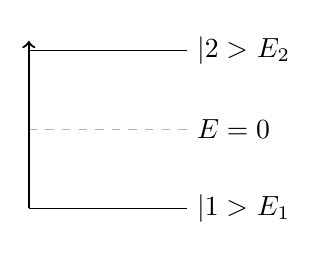
\begin{tikzpicture}
		\tikzstyle{level}=[draw=none,minimum width=2.0cm,minimum height=0.01cm]
		
		\node (A) at (0,-1) [level, label={right:$|1>$ $E_1$}]  {};
		\node (O) at (0,0) [level, label={right:$E=0$}] {};
		\node (B) at (0,1) [level, label={right:$|2>$ $E_2$}] {};
		
		\draw (A.west)--(A.east);
		\draw[dashed, opacity=0.3] (O.west)--(O.east);
		\draw (B.west)--(B.east);
		\draw[thick ,->, label={above left:$E$}] (A.west)--(B.north west);
				
		
		\end{tikzpicture}
		\caption{Átomo de dos niveles}
		\label{fig: two level}
	\end{center}
\end{figure} 

Tomando como referencia a la energía intermedia entre ambos niveles (figura \ref{fig: two level}), podemos escribir a las energías de ambos niveles    como  

\[ \begin{cases}
	E_1=-\frac{\hbar}{2}w_{21}\\
	E_2=\frac{\hbar}{2}w_{21}
\end{cases}
\]

y reemplazando en la ecuación (\ref{eq: h at 1}) ahora el hamiltoniano del átomo se escribe como 

\begin{equation}
	H_{at}=\frac{\hbar}{2}w_{21} [b^{\dagger}_2b_2-b^{\dagger}_1b_1]=\hbar w_{21} \sigma_3
	\label{eq: h at final}
\end{equation}

Donde $\sigma_3$ es la inversión de población.


\subsubsection{El Hamiltoniano del campo electromagnético}

Por otro lado, de la cuantizacion del campo electromagnético, se tiene que 

\begin{equation}
	H_c=\hbar w_{\lambda}(a^{\dagger}_{\lambda}a_{\lambda}+1/2)
	\label{eq: h electro}
\end{equation}


\subsubsection{El Hamiltoniano de interacción}

Por ultimo, si pensamos al átomo de dos niveles como un  dipolo, la interacción del dipolo con el campo electromagnético se puede escribir como 

\begin{equation}
	H_{int}=\frac{1}{2m}(\bar{p}-e\bar{A})^2+V(r)
	\label{eq: h int 1}
\end{equation}


donde puedo escribir el termino $(\bar{p}-e\bar{A})^2$ como 
\[\frac{1}{2m}(\bar{p}-e\bar{A})^2=\frac{1}{2m}(p^2+e^2A^2+e[p,A])-\frac{e}{m}\bar{p}\bar{A}
\]

Escribiendo a $\bar{A}$ en términos del campo cuantizado

\begin{equation}
\bar{A}(\bar{r})=\sum_{\lambda}\sqrt{\frac{\hbar}{2\epsilon w_{\lambda}V}} (a^{\dagger}_{\lambda}e^{i\bar{k}_{\lambda}\bar{r}}+a_{\lambda}e^{-i\bar{k}_{\lambda}\bar{r}})
\end{equation}


\begin{equation}
\bar{E}(\bar{r})=\sum_{\lambda}\sqrt{\frac{\hbar}{2\epsilon w_{\lambda}V}} (a^{\dagger}_{\lambda}e^{i\bar{k}_{\lambda}\bar{r}}+a_{\lambda}e^{-i\bar{k}_{\lambda}\bar{r}})
\end{equation}

Aproximaciones

\begin{itemize}
	\item El termino $\frac{p^2}{2m}$ se puede despreciar argumentando que cada átomo tiene una energía cinética aleatoria, por lo tanto el valor medio de la energía cinética es $0$.
	
	\item El termino $[\bar{p},\bar{A}]=-i\hbar\partial_{q}A=-i\hbar\nabla \cdot A=0 $.
	
	\item El termino $e^2\bar{A}^2=e^2\sum_{\lambda}\alpha^2_{\lambda}((a^{\dagger})^2e^{i2kr}+[a,a^{\dagger}]+(a^2e^{-i2kr})$.
	Los términos con el doble de frecuencia se desprecian por tener poca ganancia%, mientras que el anticonmutador da $0$. neceita un campo muy grande. interacc foton-foton
	
\end{itemize}
\textcolor{red}{terminar esta parte}

por lo tanto, 

\begin{equation}
	H_{int}=-\frac{e}{m}\bar{p}\bar{A}
\end{equation}

.....

\begin{equation}
	H_{int}=-\frac{e}{m}\int \sum_{\lambda j j'}b^{\dagger}_j\varphi^*_j \sqrt{\frac{\hbar}{2\epsilon w_{\lambda}V}}\bar{p} (a^{\dagger}_{\lambda}e^{i\bar{k}_{\lambda}\bar{r}}+a_{\lambda}e^{-i\bar{k}_{\lambda}\bar{r}})b_{j'}\varphi_{j'}
\end{equation}

por lo tanto las integrales se reducen a los elementos de matriz de $\bar{p}$

\begin{equation}
	p_{jj'}=m\dot x{jj'}=m[H,x]_{jj'}=\frac{im}{\hbar}(E_j-E_{j'})x_{jj'}=imw_{jj'}x_{jj'}
\end{equation}

Por lo tanto se obtiene

\begin{equation}
	H_{int}=-i\sum_{\lambda j j'} \sqrt{\frac{\hbar}{2\epsilon w_{jj'}V}}  (a^{\dagger}_{\lambda}e^{i\bar{k}_{\lambda}\bar{r}}+a_{\lambda}e^{-i\bar{k}_{\lambda}\bar{r}})    \int \varphi^*_j ex_{jj'}\varphi_{j'} b^{\dagger}_jb_{j'}
\end{equation}

donde la única integral que queda por hacer ahora es el valor medio de $ex_{jj'}$, el cual no es otra cosa que el momento dipolar clásico.


\begin{equation}
	H_{int}=-i\sum_{\lambda j j'} \sqrt{\frac{\hbar}{2\epsilon w_{jj'}V}}  (a^{\dagger}_{\lambda}e^{i\bar{k}_{\lambda}\bar{r}}+a_{\lambda}e^{-i\bar{k}_{\lambda}\bar{r}})    \langle \mu \rangle_{jj'} b^{\dagger}_jb_{j'}
\end{equation}

Planteando ahora que el sistema tiene solo dos niveles, $j,j'=1;2$

\begin{equation}
	H_{int}=-i\sqrt{ \frac{\hbar w_{21}^2}{2\epsilon V w_{\lambda} } } [....]
\end{equation}

suponiendo que ...

\begin{equation}
	H_{int}=-i\sqrt{ \frac{\hbar w_{21}^2}{2\epsilon V w_{\lambda} } }  [ \langle \mu \rangle_{21}(a^{\dagger}_{\lambda}+a_{\lambda})(b^{\dagger}_2b_{1}) + \langle \mu \rangle_{12} (a^{\dagger}_{\lambda}+a_{\lambda})(b^{\dagger}_1b_{2})  ]
\end{equation}

\[  \langle \mu \rangle_{21}=\langle \mu \rangle_{12}=\langle \mu \rangle   \]

\[\langle \mu \rangle_{11}=\langle \mu \rangle_{22}=0\]

Definiendo a la polarización como :

\begin{equation}
	\begin{cases}
		\sigma^+=b^{\dagger}_2b_{1}\\
		\sigma^-=b^{\dagger}_1b_{2}
	\end{cases}
\end{equation}

$\sigma^+$ representa la transición del estado $|1>$ al estado $|2>$, mientras que $\sigma^-$ representa la transicion del estado $|2>$ al estado $|1>$

\begin{equation}
H_{int}=-i\sqrt{ \frac{\hbar w_{21}^2}{2\epsilon V w_{\lambda} } }   \langle \mu \rangle (a^{\dagger}_{\lambda}+a_{\lambda})(\sigma^+ + \sigma^-) 
\label{eq: h int final}
\end{equation}

\subsubsection{El Hamiltoniano total y la evolución temporal}

Ahora podemos escribir el hamiltoniano total juntando los resultados obtenidos a partir de las ecuaciones (\ref{eq: h int final}), (\ref{eq: h electro}) y (\ref{eq: h at final}).

\begin{equation}
	H=\hbar w_{21} \sigma_3 + \hbar w_{\lambda}(a^{\dagger}_{\lambda}a_{\lambda}+1/2) + -i\sqrt{ \frac{\hbar w_{21}^2}{2\epsilon V w_{\lambda} } }   \langle \mu \rangle (a^{\dagger}_{\lambda}+a_{\lambda})(\sigma^+ + \sigma^-) 
\end{equation}

donde 

\begin{equation}
	\begin{cases}
		\sigma^+=b^{\dagger}_2b_{1}\\
		\sigma^-=b^{\dagger}_1b_{2}\\
		\sigma_3=\frac{1}{2}[b^{\dagger}_2b_2-b^{\dagger}_1b_1]	
	\end{cases}
\end{equation}

aplicando la ecuación de Heinsenberg para la evolución temporal de $\sigma_3$ y $\sigma^+$:

\begin{equation}
	\begin{cases}
		\partial_t \sigma^+=-\frac{i}{\hbar}[\sigma^+,H]\\

		\partial_t \sigma_3=-\frac{i}{\hbar}[\sigma_3,H]	
	\end{cases}
\end{equation}

\begin{equation}
\begin{cases}
[\sigma_3,\sigma^+]=-\sigma^+\\
[\sigma_3,\sigma^-]=-\sigma^-\\
[\sigma^+,\sigma^-]=2\sigma_3\\	
\end{cases}
\end{equation}

que son la evolución temporal de la inversión de población y de la polarización.

\begin{equation}
	\partial_t \sigma_3=-\frac{\langle \mu \rangle }{\hbar}	\sqrt{ \frac{\hbar w_{21}^2}{2\epsilon V w_{\lambda} } } \{ (a^{\dagger}\sigma^+ - a\sigma^- )+a\sigma^+ +a^{\dagger}\sigma^-   \}
\end{equation}


\textcolor{red}{Para la evolucion libre, sin interaccion los operadores evolucionarian de manera tal que }

\begin{equation}
	\begin{cases}
		a(t)=a(0)e^{iw_{\lambda}t}\\
		\sigma^+(t)=\sigma^+(0)e^{iw_0t}
	\end{cases}
\end{equation}

Por lo tanto los terminos con ambos operadores evolucionan aproximadamente de forma que 

\begin{equation}
	\begin{cases}
		a^{\dagger}\sigma^- \approx  e^{-i(w_0-w_{\lambda})t}\\
		a\sigma^+ \approx e^{i(w_0-w_{\lambda})t}\\
		a\sigma^- \approx e^{-i(w_0+w_{\lambda})t}\\
		a^{\dagger}\sigma^+ \approx e^{i(w_0+w_{\lambda})t}
	\end{cases}
\end{equation}

Lo que nos da otro argumento para despreciar los terminos no conservativos cuando $w_{\lambda} \approx w_0$ bajo la aproximacion de \textit{rotating wave}.


\begin{figure}[htc]
	\begin{center}
		
		\begin{tikzpicture}
		\tikzstyle{level}=[draw=none,minimum width=1.5cm,minimum height=0.01cm]
		\tikzstyle{snakeline} = [decorate, decoration={pre length=0.2mm,
			post length=1mm, snake, amplitude=.4mm,
			segment length=2mm}, ->]
		\tikzstyle{connector} = [->]

%%%%%%%%%%%%%%%%%%%%%%%%%%%%%%%%%%%%%%%%%%%%%%%%%%%%%%%%%%%%%%%		
		\node (A1) at (0,-1) [level,label={below: Absorcion} ]  {};
		\node (O1) at (0,0) {};
		\node (B1) at (0,1) [level,label={above:$a^{\dagger}\sigma^+$}] {};
		
		\draw (A1.west)--(A1.east);
		\draw (B1.west)--(B1.east);
		\draw[connector] (A1)--(B1);
		\draw[snakeline] ($(O1)-(1.0cm,0cm)$) -- node[above left] {$\gamma$} ++(O1);
%		\tkzLabelSegment[below=2pt](F,G){Modulador Electro Optico}
%%%%%%%%%%%%%%%%%%%%%%%%%%%%%%%%%%%%%%%%%%%%%%%%%%%%%%%%%%%%%%%			
		\node (A2) at (4,-1) [level,label={below: No conserva E} ]  {};
		\node (O2) at (4,0) {};
		\node (B2) at (4,1) [level, label={above:$a^{\dagger}\sigma^-$}] {};
		
		\draw (A2.west)--(A2.east);
		\draw (B2.west)--(B2.east);
		\draw[connector] (B2)--(A2);
		\draw[snakeline] ($(O2)-(1.0cm,0cm)$) -- node[above left] {$\gamma$} ++(O2);
%%%%%%%%%%%%%%%%%%%%%%%%%%%%%%%%%%%%%%%%%%%%%%%%%%%%%%%%%%%%%%%
		\node (A3) at (8,-1) [level,label={below: No conserva E}]  {};
		\node (O3) at (8,0) {};
		\node (B3) at (8,1) [level, label={above:$a\sigma^+$}] {};
		
		\draw (A3.west)--(A3.east);
		\draw (B3.west)--(B3.east);
		\draw[connector] (A3)--(B3);
		\draw[snakeline] (O3) -- node[above right] {$\gamma$} ++(1.0cm,0cm);
%%%%%%%%%%%%%%%%%%%%%%%%%%%%%%%%%%%%%%%%%%%%%%%%%%%%%%%%%%%%%%%
		\node (A4) at (12,-1) [level,label={below: Emision}, label={right:$|1>$}]  {};
		\node (O4) at (12,0) {};
		\node (B4) at (12,1) [level, label={above:$a\sigma^-$}, label={right:$|2>$}] {};
		
		\draw (A4.west)--(A4.east);
		\draw (B4.west)--(B4.east);
		\draw[connector] (B4)--(A4);
		\draw[snakeline,label={[above right]{$\gamma$}}] (O4) -- node[above right] {$\gamma$} ++(1.0cm,0cm);
		
		
		\end{tikzpicture}
		\caption{Interacciones del átomo de dos niveles}
		\label{fig: interacciones}
	\end{center}
\end{figure} 


\begin{equation}
	\partial_t \sigma_3=-\frac{\langle \mu \rangle }{\hbar}	\sqrt{ \frac{\hbar w_{21}^2}{2\epsilon V w_{\lambda} } } \{ a\sigma^+ + a^{\dagger}\sigma^-   \}
\end{equation}


Para la polarización:

\begin{align}
	\partial_t \sigma_+ & =-\frac{i}{\hbar}[\sigma_+,H]	 \nonumber \\
						& = iw_{21}\sigma^+ - \frac{\langle \mu \rangle }{\hbar} \sqrt{ \frac{\hbar w_{21}^2}{2\epsilon V w_{\lambda} } }    \{ [\sigma^+,a\sigma^+]+[\sigma^+,a^{\dagger}\sigma^-]   \} \nonumber \\
						& =  iw_{21}\sigma^+ - 2 \frac{\langle \mu \rangle }{\hbar} \sqrt{ \frac{\hbar w_{21}^2}{2\epsilon V w_{\lambda} } }   a^{\dagger}\sigma_3
\end{align}



Por otro lado se puede realizar la misma cuenta para $a^{\dagger}$

\begin{align}	
	\partial_t a^{\dagger} &= -\frac{i}{\hbar}[a^{\dagger},H] \nonumber \\
	&= -\frac{i}{\hbar} \{ \hbar w_{\lambda}[a^{\dagger},a^{\dagger}_{\lambda}a_{\lambda}] + -i\sqrt{ \frac{\hbar w_{21}^2}{2\epsilon V w_{\lambda} } }   \langle \mu \rangle (  [a^{\dagger},a^{\dagger}\sigma^-]  +  [a^{\dagger},a\sigma^+]  ) \}     	
\end{align}

Usando las reglas de conmutación y que $ [a^{\dagger},a]=1$

\begin{equation}
	\partial_t a^{\dagger}= -\frac{i}{\hbar} \{ \hbar w_{\lambda}a^{\dagger} + -i\sqrt{ \frac{\hbar w_{21}^2}{2\epsilon V w_{\lambda} } }   \langle \mu \rangle \sigma^+  \}     	
\end{equation}

\begin{equation}
\begin{cases}
	\partial_t a^{\dagger}=  -i w_{\lambda}a^{\dagger} + \sqrt{ \frac{\hbar w_{21}^2}{2\epsilon V w_{\lambda} } }  \frac{\langle \mu \rangle }{\hbar}	 \sigma^+    \\
	\partial_t \sigma_+ =  iw_{21}\sigma^+ - 2 \frac{\langle \mu \rangle }{\hbar} \sqrt{ \frac{\hbar w_{21}^2}{2\epsilon V w_{\lambda} } }   a^{\dagger}\sigma_3\\
	\partial_t \sigma_3=-\frac{\langle \mu \rangle }{\hbar}	\sqrt{ \frac{\hbar w_{21}^2}{2\epsilon V w_{\lambda} } } \{ a\sigma^+ + a^{\dagger}\sigma^-   \}
\end{cases}
\label{eq: quantum rates}
\end{equation}
Definiendo 

\begin{equation}
	\begin{cases}
		\mathcal{P}=\frac{1}{N}\sum_{n=1}^{N}(\sigma^+)_n\\ 
		
		D=\frac{1}{N}\sum_{n=1}^{N}(\sigma_3)_n	
\end{cases}
\end{equation}



Ahora suponemos que el medio interactua con un campo externo coherente de la forma 
\[ E_{ext}=-i \frac{\hbar w_{21}^2}{2\epsilon V w_{\lambda} }  a^{\dagger} e^{-i(kz-wt)}  \]
\textcolor{red}{chequear la cte.}
\[\bar{E}(\bar{r})=\sum_{\lambda}\sqrt{\frac{\hbar}{2\epsilon w_{\lambda}V}} a^{\dagger}_{\lambda}e^{i\bar{k}_{\lambda}\bar{r}}  \]

Por lo tanto puedo escribir a $a$ y $a^{\dagger}$ como :
\begin{equation}
\begin{cases}
\frac{\hbar w_{21}^2}{2\epsilon V w_{\lambda} } a^{\dagger} = i E_{ext} e^{i(kz-wt)}\\
\frac{\hbar w_{21}^2}{2\epsilon V w_{\lambda} }  a = -i E^*_{ext} e^{-i(kz-wt)}\\
\end{cases}
\end{equation}

Remplazando en las ecuaciones (\ref{eq: quantum rates})

\begin{equation}
	\begin{cases}
		\partial_t E_{ext}= -i \hbar w_{\lambda}a^{\dagger} + \sqrt{ \frac{\hbar w_{21}^2}{2\epsilon V w_{\lambda} } }  \frac{\langle \mu \rangle }{\hbar}	 \sigma^+ \\
		\partial_t P =  iw_{21}\sigma^+ - 2 \frac{\langle \mu \rangle }{\hbar} \sqrt{ \frac{\hbar w_{21}^2}{2\epsilon V w_{\lambda} } }   a^{\dagger}\sigma_3\\
		\partial_t D=-\frac{\langle \mu \rangle }{\hbar}	\sqrt{ \frac{\hbar w_{21}^2}{2\epsilon V w_{\lambda} } } \{ a\sigma^+ + a^{\dagger}\sigma^-   \}
	\end{cases}
	\label{eq: quantum clasic rates}
\end{equation}



\textcolor{red}{Ojo que haca hay una aprox}

\textcolor{red}{Preg: le queda complejo con esto}


\textcolor{red}{revisar las constantes y ordenar mejor lo del hamiltoniano de interacción}
